\documentclass[14pt, a4paper]{extarticle}
% Русская локализация
\usepackage[english,russian]{babel}


\usepackage{appendix}
\usepackage{alphabeta}

% Использование математических шрифтов
\usepackage{unicode-math}

% Шрифты
\usepackage{fontspec}
\usepackage{courier}
\defaultfontfeatures{Ligatures={TeX},Renderer=Basic}
\setmainfont[Ligatures={TeX}]{Times New Roman}
\setmonofont{Courier New}
\setmathfont{XITS Math}

% Расширенные ссылки
\usepackage{nameref}

% Оформление URL
\usepackage{xurl}
\usepackage{hyperref}
\hypersetup{
  colorlinks,
  citecolor=black,
  filecolor=black,
  linkcolor=black,
  urlcolor=black,
  breaklinks=true,
}
\urlstyle{same}

% Поддержка изображений
\usepackage{graphicx}
\graphicspath{{./images/}}
\DeclareGraphicsExtensions{.jpg,.png}
\usepackage{svg}

% Таблицы
\usepackage{tabularx}
\usepackage{tabulary}
\usepackage{ltablex}
\usepackage{multirow}
\usepackage{hhline}
% Выравнивание по левому краю, с многострочностью
\newcolumntype{s}{>{\raggedright\arraybackslash}X}

% Поддержка листингов
\usepackage{listings}
\lstdefinestyle{gost}{
  basicstyle=\ttfamily\footnotesize,
  breakatwhitespace=false,
  breaklines=true,
  keepspaces=true,
  showspaces=false,
  showstringspaces=false,
  frame=single
}
\lstset{style=gost}%

% Отступ первой строки первого абзаца
\usepackage{indentfirst}
\linespread{1.25}

% Размер полей в документе
\usepackage{geometry}
\geometry{left=3cm}
\geometry{right=1cm}
\geometry{top=2cm}
\geometry{bottom=2cm}

% Абзацный отступ
\setlength{\parindent}{1.25cm}

% Отступ для элементов в списке
\usepackage{enumitem}
\setlist{left=\parindent, labelsep=1cm, itemsep=0pt, topsep=0pt}

% Загрузка pdf-документов (нужно для титульных листов)
\usepackage[final]{pdfpages}
% Возможность поворота pdf файло
\usepackage{pdflscape}
\usepackage{everypage}

\newcommand{\Lpagenumber}{\ifdim\textwidth=\linewidth\else\bgroup%
    \dimendef\margin=0 %use \margin instead of \dimen0
    \ifodd\value{page}\margin=\oddsidemargin
    \else\margin=\evensidemargin%
    \fi

\raisebox{\dimexpr-\topmargin-\headheight-\headsep-0.5\linewidth}[0pt][0pt]{%
      \rlap{\hspace{\dimexpr-\margin+\textheight+\footskip}%
        \llap{\rotatebox{90}{\thepage}}}}%
    \egroup\fi}
\AddEverypageHook{\Lpagenumber}%

\usepackage{float}
% Форматирование подписей
\usepackage{caption}

\usepackage{newfloat}
% \DeclareCaptionType{listing}

\DeclareCaptionLabelSeparator{emdash}{\;\textemdash\;}
\captionsetup[figure]{name={Рисунок}, labelsep=emdash, justification=centering,
position=above, singlelinecheck=off, font={small, bf}, labelfont=bf, skip=6pt}
\captionsetup[table]{name={Таблица}, labelsep=emdash,
justification=raggedright, position=top, singlelinecheck=off, font={small, it},
labelfont=it, skip=6pt, margin=0cm}
% \captionsetup[lstlisting]{labelsep=emdash, justification=raggedright,
% position=top, singlelinecheck=off, font={small, it}, labelfont=it, skip=6pt,
% margin=0cm}

% Нумеровать внутри заголовков первого уровня
\counterwithin{figure}{section}
\counterwithin{table}{section}
% \counterwithin{lstlisting}{section}
\AtBeginDocument{\counterwithin{lstlisting}{section}}

% Отключение переносов текста
\usepackage{ragged2e}
\justifying
\tolerance=500
\hyphenpenalty=10000
\emergencystretch=3em

% Форматирование заголовков
\usepackage{titlesec}
% Оформление заголовка первого уровня
% Полужирное начертание
% Кегль 18 пт
% С новой страницы
\titleformat{\section}[block]
{\newpage\bfseries\fontsize{18pt}{21.6pt}\selectfont}
{\thesection}
{1em}{}
% Оформление ненумерованных заголовков (Введение, Содержание, список
% источников, и.т.д.)
\titleformat{name=\section,numberless}[block]
{\centering\newpage\bfseries\fontsize{18pt}{21.6pt}\selectfont}
{}
{0em}{}{}
% Отступы у заголовков первого уровня
\titlespacing{\section}
{\parindent}% отступ слева (равен 1.25 см, как у отступа первой строки абзаца)
{0em}% интервал перед
{10mm}% интервал после
% Оформление заголовков второго уровня
\titleformat{\subsection}[block]
{\bfseries\fontsize{16pt}{19.2pt}\selectfont}
{\thesubsection}
{1em}{}
% Отступы у заголовков второго уровня
\titlespacing{\subsection}
{\parindent}% пробел слева
{15mm}% отступ перед
{10mm}% отступ после
% Оформление заголовков второго уровня
\titleformat{\subsubsection}[block]
{\bfseries\selectfont}
{\thesubsection}
{1em}{}
% Отступы у заголовков второго уровня
\titlespacing{\subsubsection}
{\parindent}% пробел слева
{15mm}% отступ перед
{10mm}% отступ после

% Оформление заголовков в содержании
\usepackage{titletoc}
\contentsmargin{0pt}
\renewcommand\contentspage{\thecontentspage}
\dottedcontents{section}[2.3em]{}{2.3em}{5pt}
\dottedcontents{subsection}[2.3em]{}{2.3em}{5pt}
% Оформление приложений
\usepackage{appendix}
\renewcommand\appendixpagename{ПРИЛОЖЕНИЯ}

% Подключение biblatex, с использованием стиля gost-numeric
\usepackage[
citestyle=gost-numeric,
style=gost-numeric,
blockpunct=emdash,
backend=biber,
sorting=none
]{biblatex}
% Запрет разрыва url ссылок
\defcounter{biburlnumpenalty}{3000}
\defcounter{biburlucpenalty}{6000}
\defcounter{biburllcpenalty}{9000}
% Добавление полей для ссылок и даты обращения к ним
\DeclareFieldFormat{url}{Режим доступа: #1}
\DeclareFieldFormat{urldate}{(Дата обращения: #1)}
\renewcommand*{\entrysetpunct}{\par\nopunct\!\!}
% Использовать prac.bib как источник
\addbibresource{diploma.bib}
% Форматирование заголовка библиографии
\defbibheading{bibliography}[\bibname]{%
  \section*{\centering #1}%
  \markboth{#1}{#1}}


\usepackage{lipsum}

\begin{document}
\def\contentsname{СОДЕРЖАНИЕ}

% Загрузка титула
\pagenumbering{gobble}
%\begin{titlepage}
%  
\includepdf{title}
%  \includepdf[pages={1-2}]{zadanie}
%\end{titlepage}
\pagenumbering{arabic}
\setcounter{page}{4}
% Содержание
\tableofcontents

\section*{ВВЕДЕНИЕ}
\phantomsection
\addcontentsline{toc}{section}{ВВЕДЕНИЕ}

Исследуемым объектом в рамках дипломной работы является ИТ-инфраструктура,
поддерживающая модуль потребительского кредитования. Этот модуль включает в
себя ответственность за управление ипотечными и кредитными продуктами, так же
за хранение и обработку данных клиентов и генерацию отчетов, как по клиентам
так и работе модуля.

Функции и задачи выполняемые модулем потребительского кредитования:
\begin{enumerate}
	\item Управление такими данными клиентов, как личная информация, кредитная
история и финансовое состояние.
	\item Обработка заявок на выдачу ипотек и кредитов. Обработка заявок включает
в себя обработку документов и оценку кредитоспособности.
	\item Выдача, обслуживание, управление платяжами и дефолтами.
	\item Мониторинг портфелей кредиторов и управление рисками.
	\item Подготовка отчетов для менеджмента и регуляторов.
\end{enumerate}

Данные, обрабатываемые ИТ-инфраструктурой модуля потребительского кредитования
включают в себя личные и финансовые данные клиентов, информацию об объектах
кредитования, таких как недвижимость для ипотеки и автомобили для автокредитов,
условия и сроки заявок на кредиты, транзакционные данные, такие как выплаты и
комиссии, данные для поддержания KYC и AML, оценки рисков и соблюдения
нормативных требований.

ИТ-инфраструктура безопасного, масштабируемого и надежного модуля
потребительского кредитования должна обеспечивать следующую перечень
требований:

\begin{enumerate}
	\item Хранение больших объемов данных без потери точности.
	\item Защиту данных с соответствием законам Российской Федерации о защите
данных (№152-ФЗ <<О персональных данных>>).
	\item Интеграция с такими банковскими системами, как CRM и AML.
	\item Резервирование хранилищ и резервное копирование.
\end{enumerate}

Проектирование и функциональное моделирование ИТ-инфраструктуры, обеспечивающей
хранение и обработку данных модуля поддержки потребительского кредитования
информационной системы кредитной организации

\section*{ГЛОССАРИЙ}
\phantomsection
\addcontentsline{toc}{section}{ГЛОССАРИЙ}
\begin{raggedright}
	ПАО --- Публичное акционерное общество. \\
	ИТ --- Информационные технологии. \\
	KYC --- Know your customer (знай своего клиента). \\
	AML --- Anti-money laundering (борьба с отмыванием денег). \\
	АКБ --- Акционерный коммерческий банк. \\
	НПФ --- Негосударственный пенсионный фонд. \\
	DFD --- \\
	BPMN --- \\
	UML --- \\
\end{raggedright}

\section{ИСХОДНЫЕ ДАННЫЕ И ПОСТАНОВКА ЗАДАЧИ}

\subsection{Характеристика объекта исследования}

Характеристика объекта исследования позволит сформировать детальное понимание о
деятельности исследуемого объекта, о том какие бизнес-процессы существуют в
компании и в модуле потребительского кредитования. Этот пункт даст понимание о
состоянии компании на рынке и раскроет ключевые метрики на основе со
оставляет конкуренцию другим других банком занимающимся потребительским
кредитованием.

АКБ <<Абсолют Банк>> (ПАО) успешно функционирует на Российском рынке с момента
своего основания 22 апреля 1993 года. За годы своей деятельности банк добился
доверия клиентов благодаря стабильности, инновационным банковским продуктам и
высокому уровню сервиса. С 2007 по 2012 годы контрольным паке том акций банка
владел <<KBC Group>>, которая приобрела 92.5\% акций за 1 млрд долларов. Однако
в настоящее время пакет акций был приобретен компаниями управляющими резервами
НПФ <<Благосостояние>>. Другой акционер — Международная Финансовая Корпорация
(IFC), владеющая пакетом в 5\% акций. Банк специализируется на ипотечном
кредитовании, автокредитовании, обслуживании малого и среднего бизнеса и
приват-банкинге, фокусируется на корпоративном финансировании и торговом
финансировании. Офисы банка представлены в 30 городах России, а центральное
отделение находится в Москве. Активы банка на конец 2024 года составили 289.2
млрд рублей, а кредитный портфель банка вырос на 10\%. Абсолют Банк активно
развивает цифровые технологии и предлагает удобные онлайн-сервисы для
управления финансами и потребительского кредитования. На Рисунке
\ref{fig:кредитный_портфель_банков_крупные} представлена динамика
изменений кредитного портфеля крупнейших банков России \cite{banks-rating}.

\begin{figure}[H]
	\centering
	\includegraphics[width=\textwidth]{кредитный_портфель_банков_крупные}
	\caption{Динамика изменений кредитного портфеля крупных банков РФ}
	\label{fig:кредитный_портфель_банков_крупные}
\end{figure}

На Рисунке \ref{fig:кредитный_портфель_банков_малые} представлена динамика
изменений кредитного портфеля банков России, которые находятся в конкуренции с
АКБ <<Абсолют Банк>>.

\begin{figure}[H]
	\centering
	\includegraphics[width=\textwidth]{кредитный_портфель_банков_малые}
	\caption{Динамика изменений кредитного портфеля банков РФ}
	\label{fig:кредитный_портфель_банков_малые}
\end{figure}

Функции модуля потребительского кредитования АКБ <<Абсолют Банк>> типичны для
банковского сектора и включают в себя следующее. Основной функций, которая
охватывает работу с данными является управление данными клиентов. Хранение
такой личной информации клиентов, так имя, адрес, контакты. Хранение данных о
расходах и доходах и кредитной истории. Такие данные применяются для оценки
кредитоспособности и соблюдения требований KYC и AML, что является
необходимостью для предотвращения финансовых преступлений.

Отдельной функцией в потребительском кредитовании является обработку заявок на
кредиты -- это прием и проверка заявок на ипотеку, кредиты и автокредиты,
которая требует верификации документов, оценку кредитного риска и определение
условий кредитования. В условия кредитования входят такие параметры, как сумма,
процентная ставка и срок. Обработка заявок на кредитование включает в себя
процесс запроса дополнительных документов в случае недостатка информации по
тем, которые запрашиваются автоматически для всех кредиторов. Одним из
процессов является применение моделей кредитного скоринга и использование
данных кредитных бюро для анализа кредитоспособности кредитора. В случае с
ипотеками проводится оценка недвижимости для определения ее рыночной стоимости.
<<Абсолют Банк>> позволяет клиентам подавать заявки на кредитование с
использованием онлайн-ресурсов и в отделении банка. На данный момент можно
заметить недостаточно оптимизированные процессы для создания и обработки заявок
с использованием онлайн-портала, так как крупные банки у которых эти процессы
оптимизированы имеют кредитный портфель многократно превышающий портфель банка
<<Абсолют>>.

Одной из основных функцией является выдача кредитов. Процесс выдачи для ипотек
считается завершенным на стадии, где заемщик подписывает документы и получает
ключи от недвижимости, а для других методов кредитования в момент когда
средства переведены на счет заемщика.

Функция обслуживания состоит из перевода средств
заемщику и управления процессом погашения выданных кредитов, что включает в
себя обработку платежей, отслеживание просрочек и работу с дефолтами. Банк
отслеживает своевременность выполнения платежей и отслеживает просроченные
задолженности, в случае просроченных задолженностей банк держит за собой право
инициировать процедуру реструктуризации долга, взыскания или передачи долга в
коллекторское агентство. Это требует эффективных систем для мониторинга и
управления рисками.

Управление рисками -- это процесс, где применяются методы
мониторинга портфелей и финансов кредиторов. Управление рисками подразумевает
проведение стресс-тестов и внедрение мер по их снижению, таких как страхование
и залог. Процесс первичной оценки рисков производится с использованием
скоринговых моделей и мониторинга портфелей, как до выдачи кредита, так и после
выдачи. Рыночные же риски, которые могут быть связаны с изменениями процентных
ставок или валютных курсов решаются с использованием хеджирования и других
финансовых инструментов.

Важнейшим бизнес процессом в банках является генерация отчетности о финансовых
результатах, анализе рисков и производительности различных подразделений,
которые могут применяться менеджментом для принятия стратегических решений.
Финансовые отчеты о балансах, прибылях и убытках предоставляются акционерам и
регуляторам. Отчеты для центрального банка России показывают данные о кредитных
портфелях и соблюдении нормативов.

АКБ <<Абсолют Банк>> обрабатывает такие типы данных, как личная информация,
финансовая история и документы. Данные об объектах кредитования, такие как
адрес, стоимость и отчеты об оценке для ипотек и марка, модель и цену для
автокредитов. Данные о заявках на кредитование, такие как цель, срок,
процентная ставка, графики платежей. Транзакционные данные, которые
подразумевают информацию о платежах, комиссиях и штрафах за просрочку. Рейтинги
рисков, информация о залоге, результаты стресс-тестов кредиторов и регуляторные
данные, которые состоят из отчетов Центральному банку РФ.

\subsection{Предпроектное обследование объекта исследования}

Обследование объекта исследования -- это важный этап, который позволит
собрать, а в результате и визуализировать информацию о текущем состоянии
ИТ-инфраструктуры модуля потребительского кредитования ПАО <<Абсолют Банк>>. В
этом пункте будут рассматриваться модели бизнес-процессов <<как есть>> в
нотации BPMN 2.0, диаграммы UML вариантов использования и DFD, на основе
анализа будут вынесены формальные и неформальные требования к улучшенной
ИТ-инфраструктуре.

На текущий момент бизнес процесс выдачи кредита через веб-приложение включает в
себя четыре актора, а ключевыми являются клиент, менеджер и кредитный
специалист. Эти акторы осуществляют действия по сопровождению, анализу
кредитоспособности, обращению в кредитное бюро и принятию решения по выдаче
кредита. Одним из внешних акторов является аудитор без которого в силу законов
РФ процесс выдачи кредита потребителю не был бы сформирован полностью, так как
для выдачи потребительских кредитов информацию о кредиторах, сроках и ставках
нужно передавать кредитору. На Рисунке\;\ref{fig:uml_use_case} изображена UML
диаграмма вариантов использования бизнес-процесса выдачи кредита.

\begin{figure}[H]
	\centering
	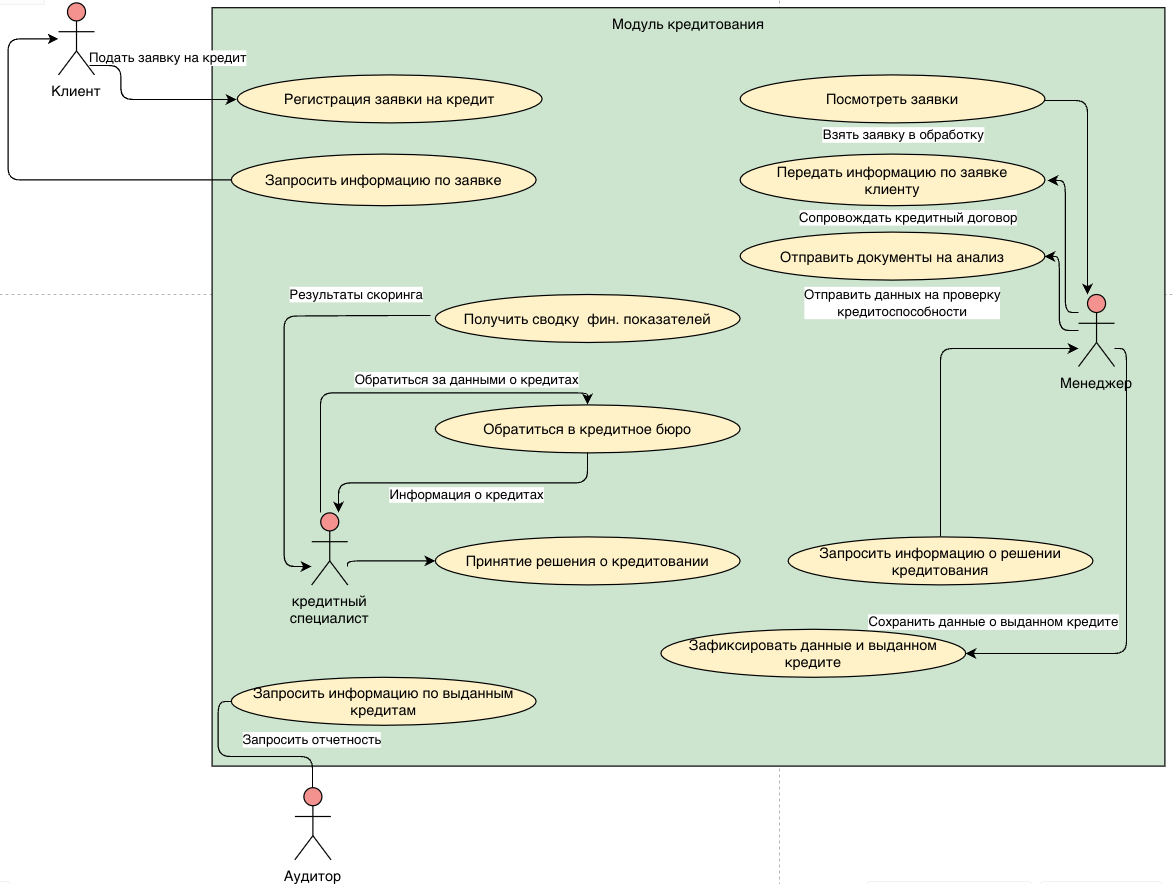
\includegraphics[width=\textwidth]{uml_use_case_extended}
	\caption{Диаграмма UML вариантов использования процесса кредитования}
	\label{fig:uml_use_case}
\end{figure}

Текстовое описание UML диаграммы вариантов использования представлена в Таблице
\ref{tab:table_use_case}

\begin{tabularx}{\textwidth}{|l|X|X|}
	\captionsetup{margin=-14pt}
	\caption{Текстовое описание вариантов использования\label{tab:table_use_case}}
		\\
	\endfirsthead
	\caption*{Продолжение таблицы~\ref{tab:table_use_case}} \\
	\hline
	№ & Актор 		       	  & Действие 					 				  \\\hline
	\endhead
	\endfoot
	\endlastfoot

	\hline
	№  & Актор 				  & Действие 					 				  \\\hline
	1  & Клиент 			  & Регистрация заявки на кредит  				  \\\hline
	2  & Клиент 			  & Запросить информацию по заявке 				  \\\hline
	3  & Менеджер 			  & Посмотреть заявки на кредит   				  \\\hline
	4  & Менеджер 			  & Передать информацию по заявке клиенту   	  \\\hline
	5  & Менеджер 			  & Отправить документы на анализ   			  \\
	6  & Менеджер 			  & Запросить информацию о решении кредитования   \\\hline
	7  & Менеджер 			  & Зафиксировать данные о выданном кредите   	  \\\hline
	8  & Кредитный специалист & Получить сводку финансовых показателей клиента\\\hline
	9  & Кредитный специалист & Обратиться в кредитное бюро 				  \\\hline
	10 & Кредитный специалист & Принять решение о кредитовании 			 	  \\\hline
	11 & Аудитор 	 		  & Запросить информацию по выданным кредитам 	  \\\hline
\end{tabularx}

Проанализировав диаграмму вариантов использования можно понять, что
бизнес-процесс выдачи кредитов с использованием веб-приложения находится на
высоком уровне цифровизации, но стоит обратить внимание на большое количество
действий, которые выполняются кредитным специалистом. Из действий выполняемых
кредитным специалистом можно избавиться от обращения в кредитное бюро
автоматизацией и вынесением этого в интеграцию с собственной CRM системой. Так
же можно избавиться от действия фиксации данных о выданном кредите, которое
выполняется актором <<менеджер>>, так как данные можно фиксировать в процессе
передачи между акторами.

На Рисунке \ref{fig:dfd0} представлена контекстная диаграмма
процесса создания заявки на кредитование клиентом через интерфейс
веб-приложения с применением нотации DFD (диаграмма потоков данных). На
Рисунке \ref{fig:dfd1} представлена декомпозиция контекстной диаграммы. На
декомпозированной диаграмме показаны основные потоки данных поступающих от
клиента, используемых внутри модуля и так же их передача за рамки модуля в
кредитное бюро для получения истории кредитов клиента, что необходимо для
точного определения кредитоспособности. Можно увидеть, что за каждым новым
запросом клиента нужно передать заявки в систему скоринга, что можно
оптимизировать сохранением результатов скоринга и в будущем при повторном
обращении через небольшое время вместо проведения повторного скоринга
воспользоваться результатами уже проведенного скоринга.

\begin{figure}[H]
	\centering
	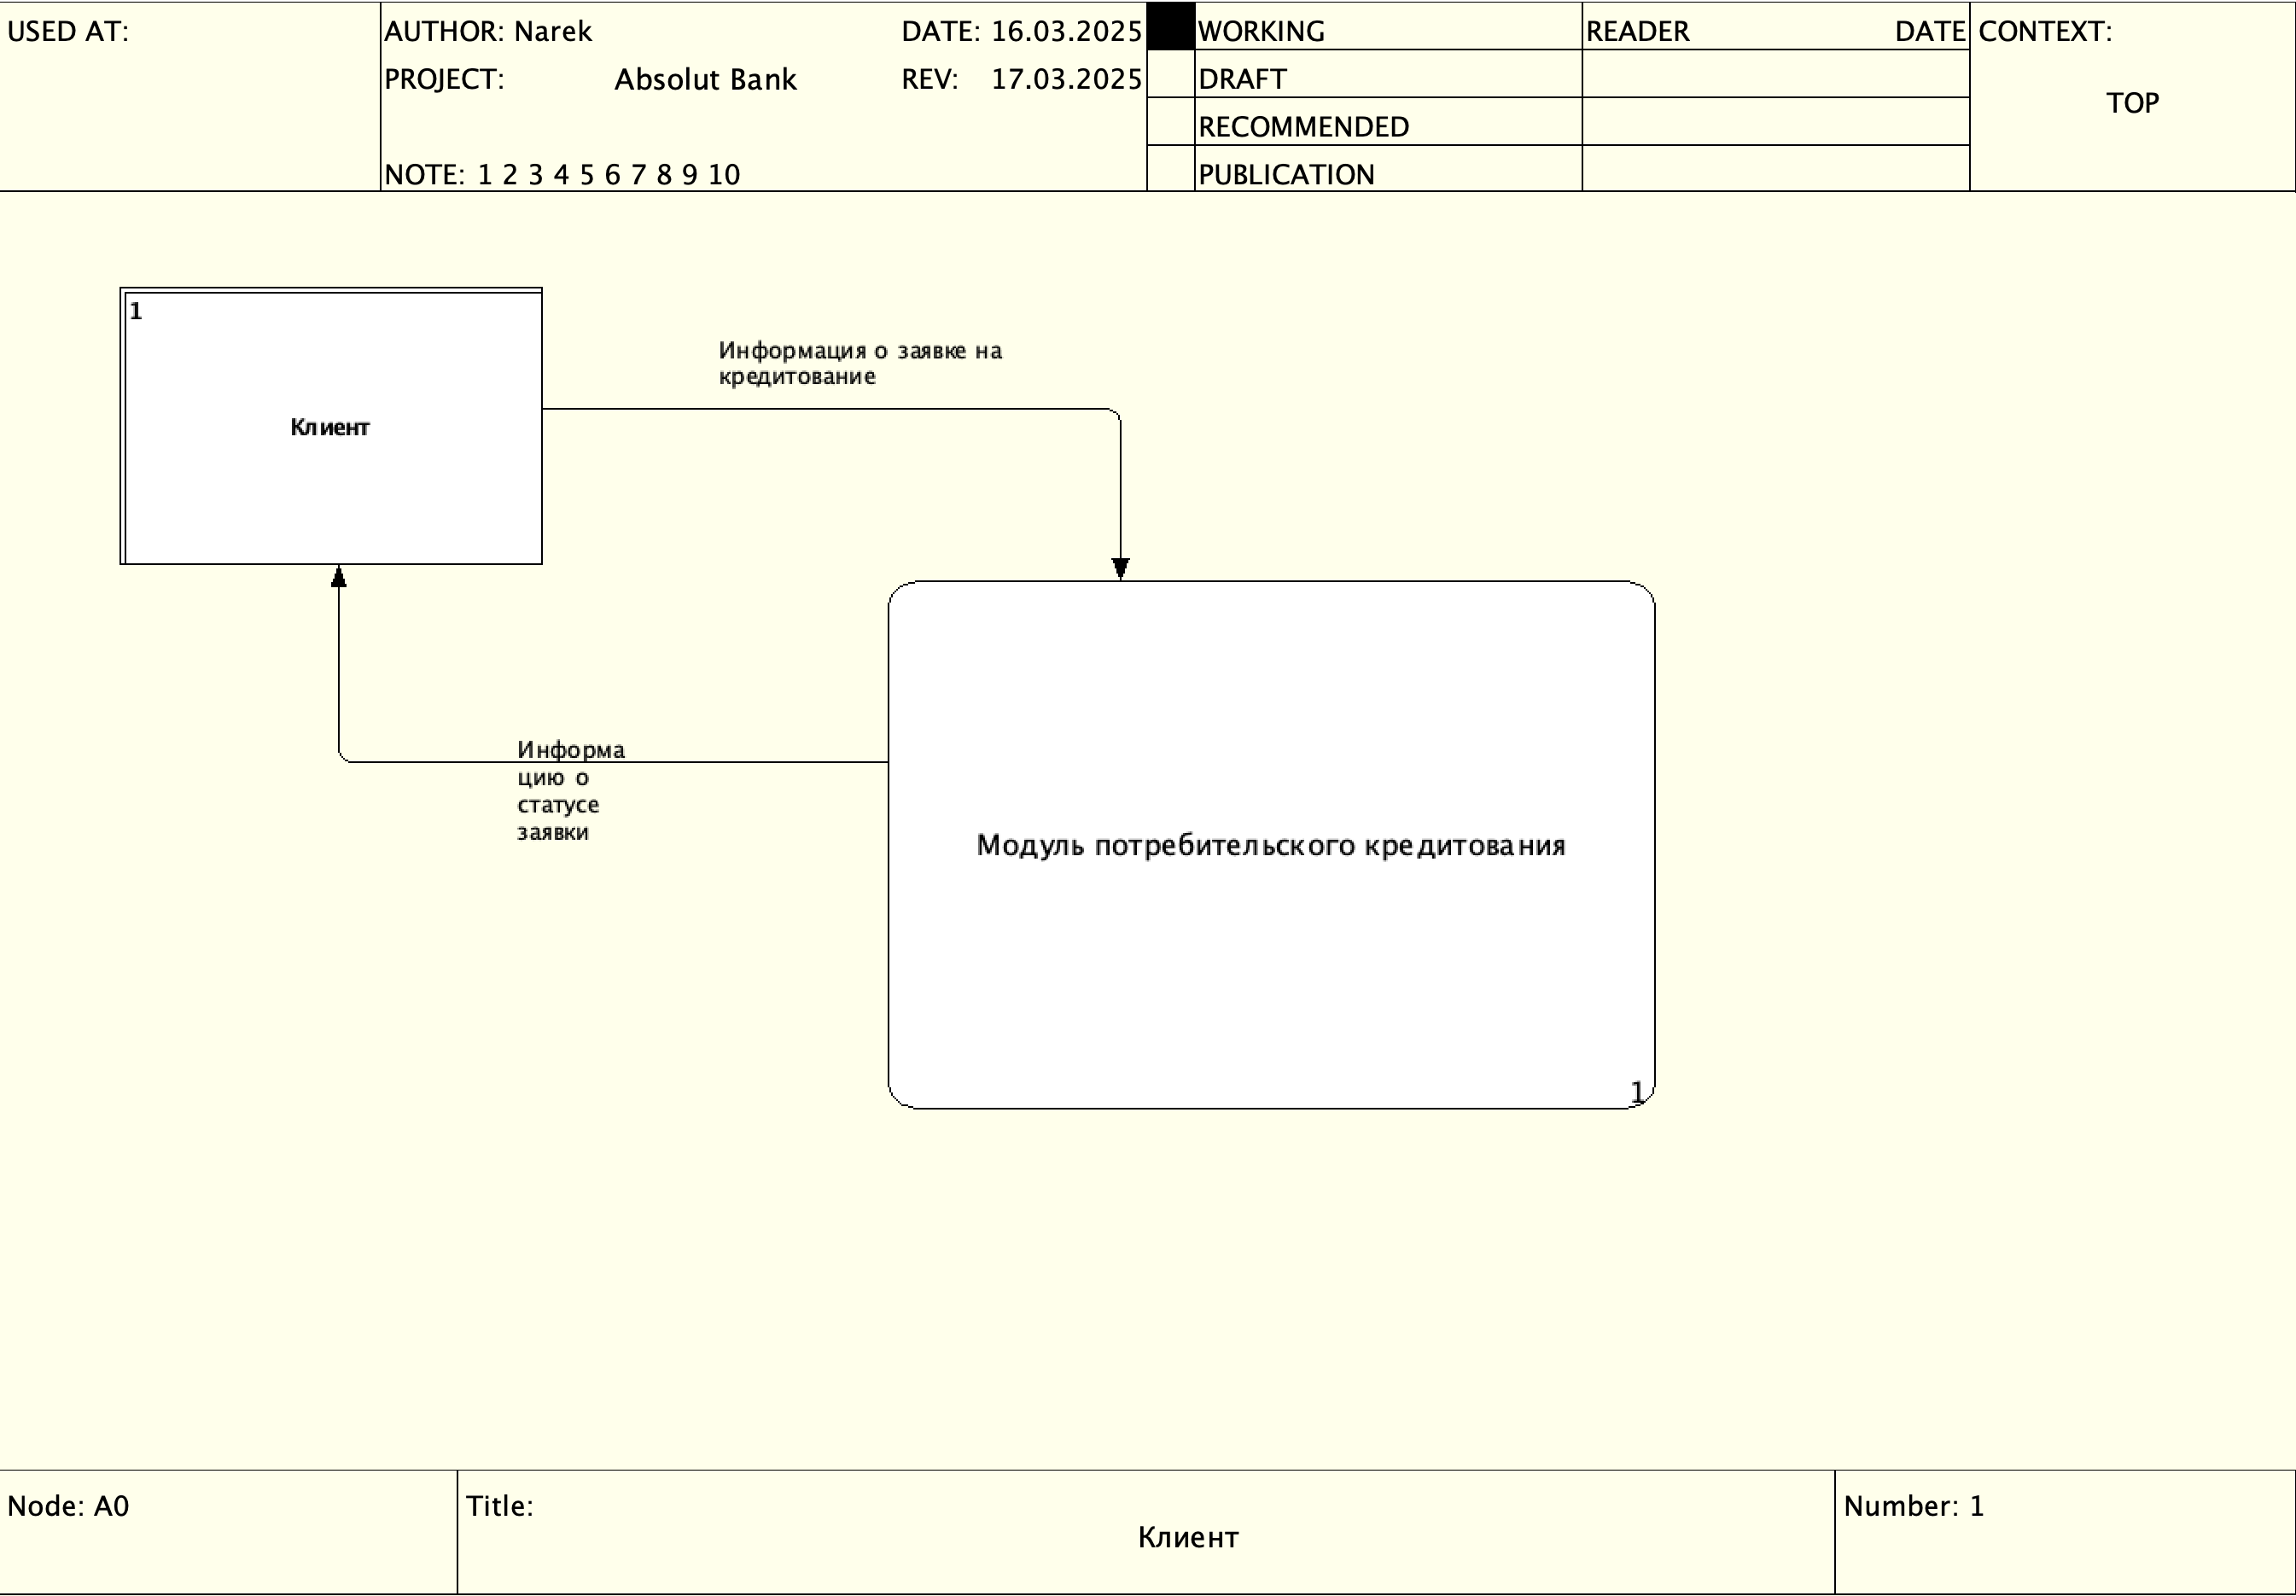
\includegraphics[scale=0.33]{dfd0}
	\caption{Контекстная диаграмма DFD процесса создания заявки на кредитование}
	\label{fig:dfd0}
\end{figure}

\begin{figure}[H]
	\centering
	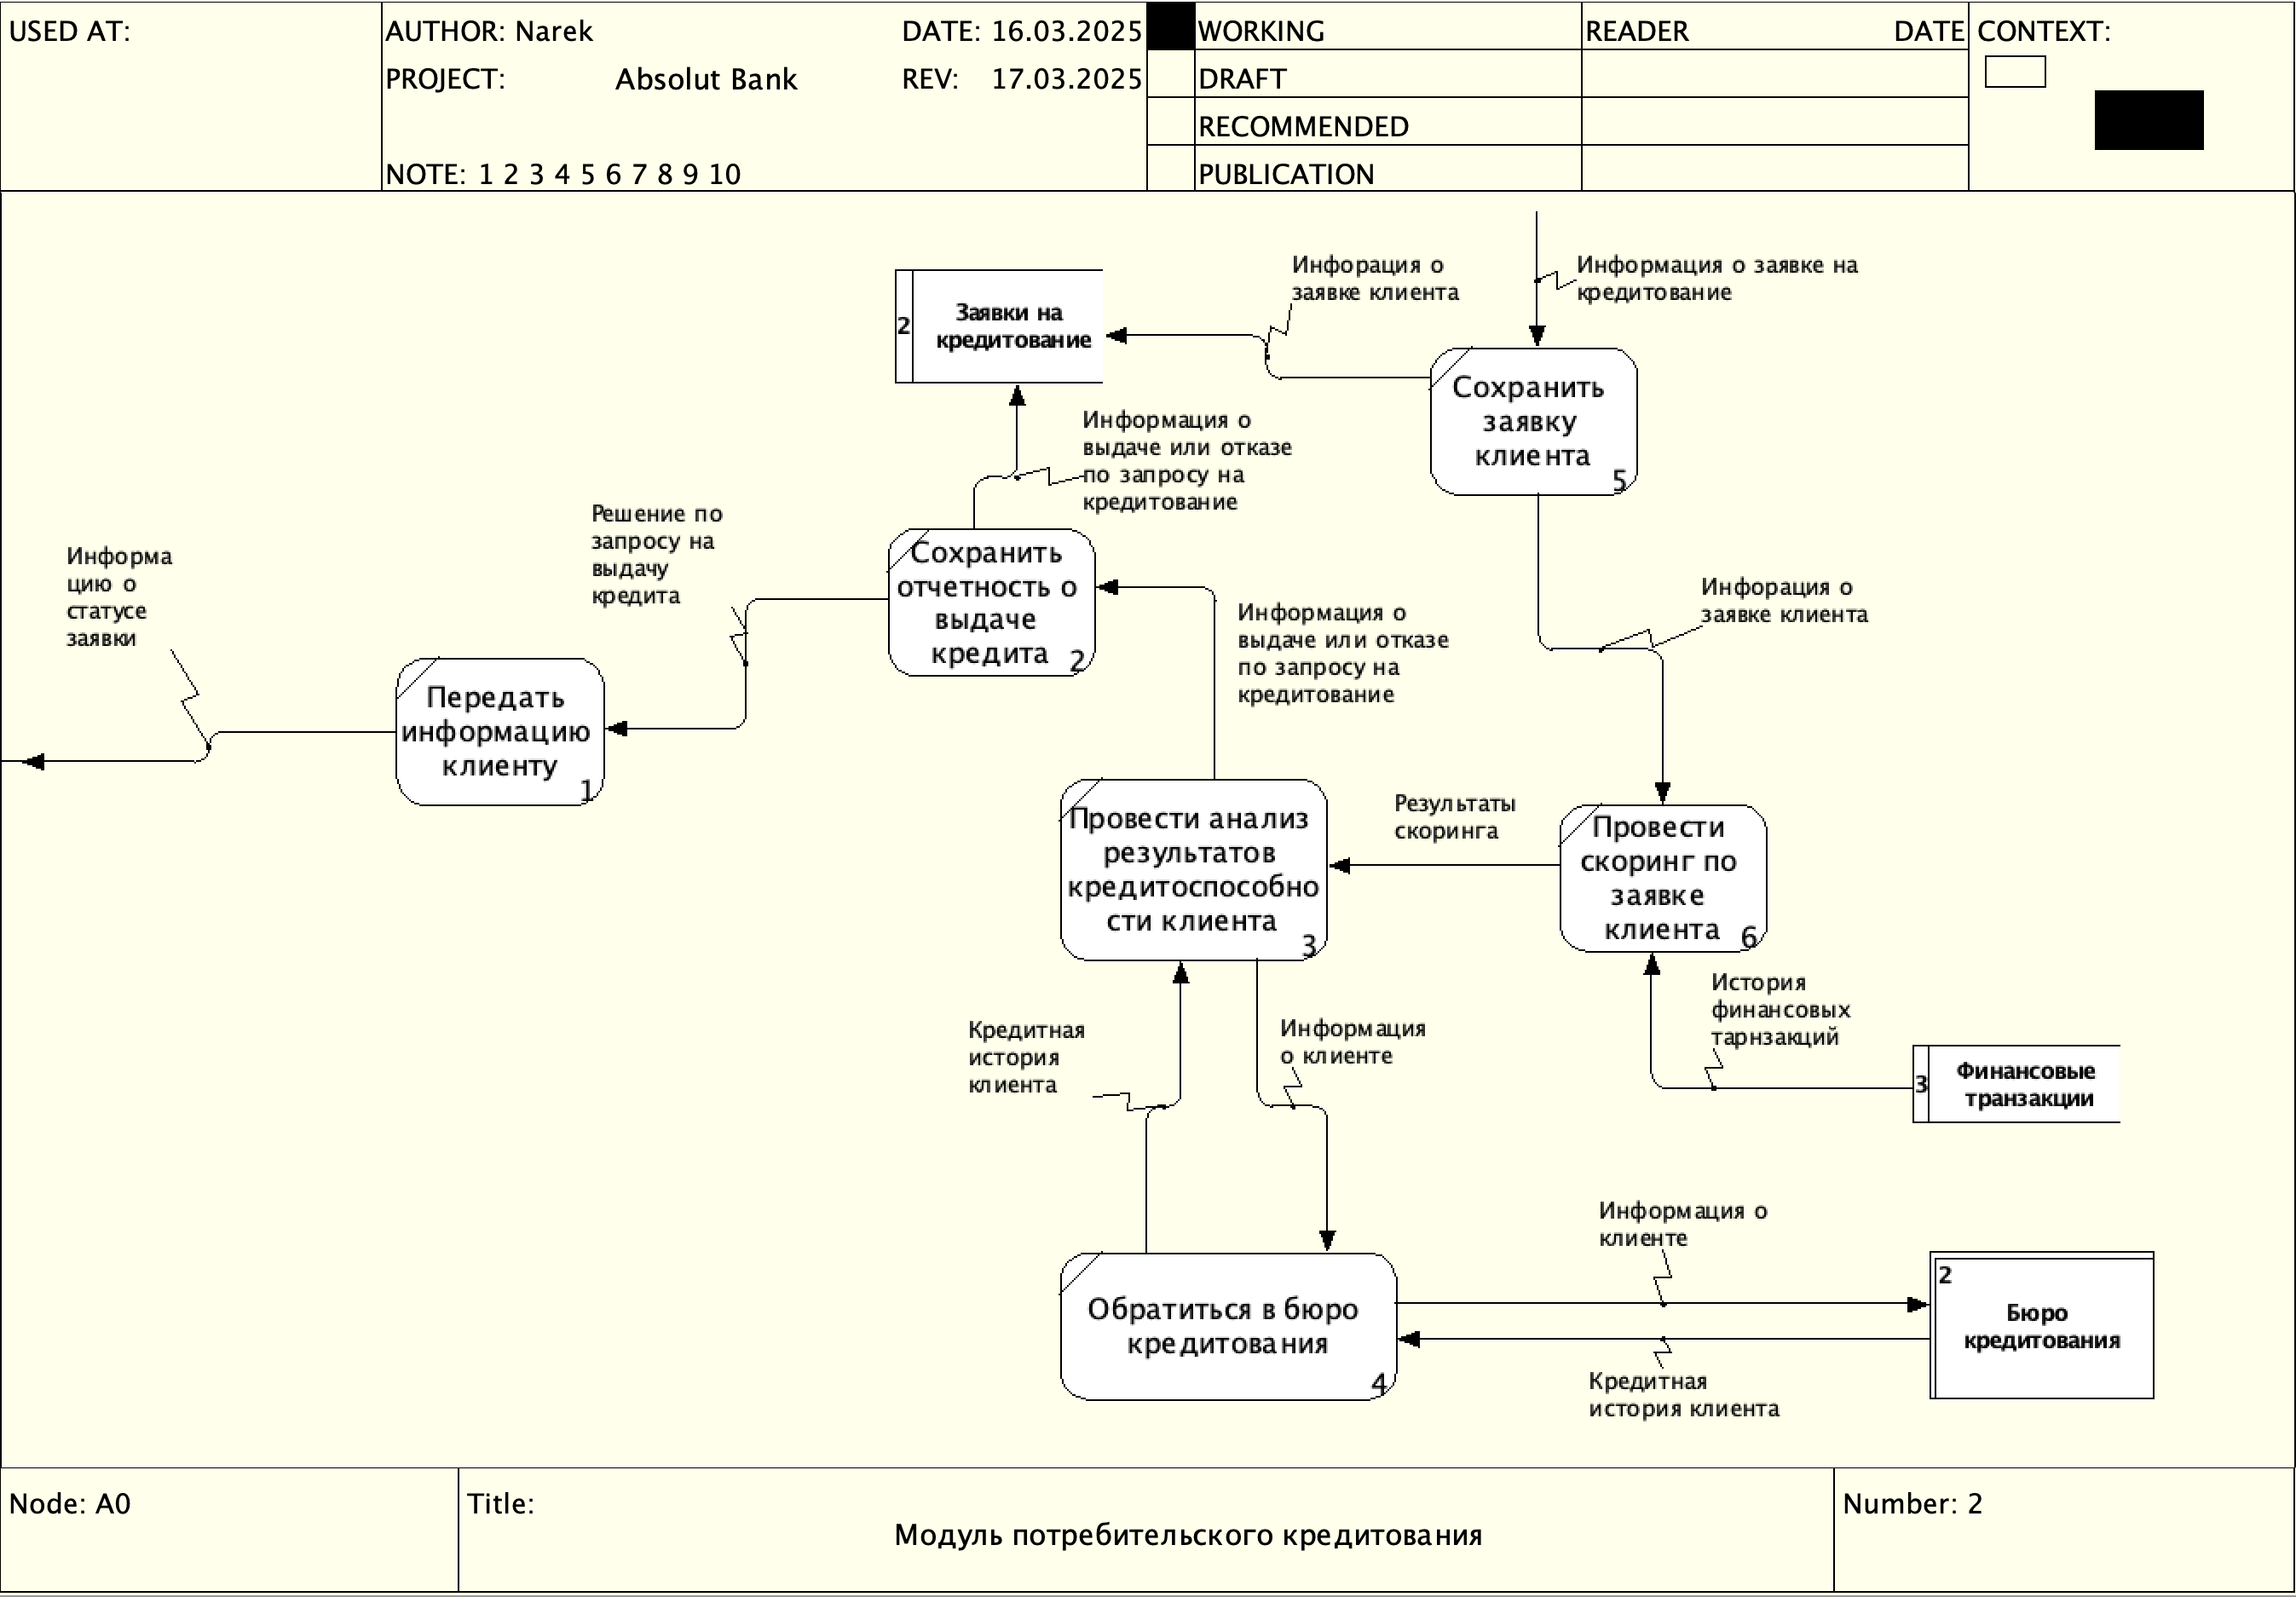
\includegraphics[scale=0.33]{dfd1}
	\caption{Декомпозиция контекстной диаграммы DFD процесса создания заявки на
кредитование}
	\label{fig:dfd1}
\end{figure}

Компоненты ИТ-инфраструктуры и технологии, которые в фокусе модуля
потребительского кредитования АКБ <<Абсолют Банк>> включают в себя системы баз
данных, системы и средства обеспечения безопасности, функциональные модули,
интеграции и пользовательский интерфейс.

АКБ <<Абсолют банк>> для хранения данных использует SQL хранилище данных,
такое как <<Oracle Database>>, и NoSQL хранилище <<MongoDB>>. Для мониторинга
компания используется и сбора метрик модуль использует программное обеспечение
<<Yandex metrica>>\;\cite{absolut-infrastructure-usage} и для системных
показателей <<Zabbix>>. Основным инструментом для бизнес-аналитики в компании
является ПО <<Power BI>>. Системы управления
кредитами, так как скоринговая  система, система верификации, система расчета
кредитного лимита у компании свои, то есть в правлении кредитами компания не
пользуется готовыми решениями. Инструменты для управления рисками у компании
так же свои, готовые решения в этом блоке компания не использует. CRM система
и весь остальной комплекс инструментов для автоматизации части
бизнес процессов, маркетинговых коммуникаций и обработки лидов
продаж используется <<BPMSoft>>\;\cite{BPMSoft-usage}. Для обеспечения
безопасности инфраструктуры используется ПО от производителя Positive
Tecnologies <<MaxPatrol>>\;\cite{absolut-MaxPatrol-usage}. Так как в банковском
секторе требуется возможность иметь интеграцию с больших количеством
сервисов и получать информацию от них, для этого нужен мощный инструмент
обеспечивающий скорость интеграции, для этого используется ПО <<BidSwitch>>.

АРМ работников офиса клиентской поддержки блока кредитования представляют из
себя компьютеры средней мощности достаточной для обработки заявок, которые
подаются клиентами в офисе. Характеристики АРМ представлены на Таблице \;

\begin{tabularx}{\textwidth}{|l|X|X|X|}
	\captionsetup{margin=-14pt}
	\caption{Текстовое описание вариантов использования\label{tab:arm_software}}
		\\
	\endfirsthead
	\caption*{Продолжение таблицы~\ref{tab:arm_software}} \\
	\hline
	№  & Компонент 		       & Модель 				& Характеристики \\\hline
	\endhead
	\endfoot
	\endlastfoot

	\hline
	№  & Компонент 		       & Модель 				& Характеристики \\\hline
	1  & Процессор 			  & Регистрация заявки на кредит  				  \\\hline
	2  & ОЗУ 			  & Запросить информацию по заявке 				  \\\hline
	3  & Хранилище 			  & Посмотреть заявки на кредит   				  \\\hline
	4  & Интернет 			  & Передать информацию по заявке клиенту   	  \\\hline
	4  & Видеокарта           &
\end{tabularx}


\subsection{Характеристика предмета исследования}



\subsection{Архитектура объекта исследования}



\subsection{Резюме проекта}

% used resources list
\begingroup
	\let\itshape\upshape
	\sloppy
	\raggedright
	\printbibliography[title=СПИСОК ИСПОЛЬЗУЕМЫХ ИСТОЧНИКОВ]
	\phantomsection
	\addcontentsline{toc}{section}{СПИСОК ИСПОЛЬЗУЕМЫХ ИСТОЧНИКОВ}
\endgroup
% used resources list

\end{document}
